% XeLaTex
%\documentclass[review]{cvpr}
\documentclass[final]{cvpr}

\usepackage[UTF8]{ctex}

%\usepackage{cvpr}
\usepackage{times}
\usepackage{epsfig}
\usepackage{graphicx}
\usepackage{amsmath}
\usepackage{amssymb}
\usepackage{subfigure}
\usepackage{overpic}

\usepackage{enumitem}
\setenumerate[1]{itemsep=0pt,partopsep=0pt,parsep=\parskip,topsep=5pt}
\setitemize[1]{itemsep=0pt,partopsep=0pt,parsep=\parskip,topsep=5pt}
\setdescription{itemsep=0pt,partopsep=0pt,parsep=\parskip,topsep=5pt}


\usepackage[pagebackref=true,breaklinks=true,colorlinks,bookmarks=false]{hyperref}


%\cvprfinalcopy % *** Uncomment this line for the final submission

\def\cvprPaperID{159} % *** Enter the CVPR Paper ID here
\def\confYear{CVPR 2020}
\def\httilde{\mbox{\tt\raisebox{-.5ex}{\symbol{126}}}}

\newcommand{\cmm}[1]{\textcolor[rgb]{0,0.6,0}{CMM: #1}}
\newcommand{\todo}[1]{{\textcolor{red}{\bf [#1]}}}
\newcommand{\alert}[1]{\textcolor[rgb]{.6,0,0}{#1}}

\newcommand{\IT}{IT\cite{98pami/Itti}}
\newcommand{\MZ}{MZ\cite{03ACMMM/Ma_Contrast-based}}
\newcommand{\GB}{GB\cite{conf/nips/HarelKP06}}
\newcommand{\SR}{SR\cite{07cvpr/hou_SpectralResidual}}
\newcommand{\FT}{FT\cite{09cvpr/Achanta_FTSaliency}}
\newcommand{\CA}{CA\cite{10cvpr/goferman_context}}
\newcommand{\LC}{LC\cite{06acmmm/ZhaiS_spatiotemporal}}
\newcommand{\AC}{AC\cite{08cvs/achanta_salient}}
\newcommand{\HC}{HC-maps }
\newcommand{\RC}{RC-maps }
\newcommand{\Lab}{$L^*a^*b^*$}
\newcommand{\mypara}[1]{\paragraph{#1.}}

\graphicspath{{figures/}}

% Pages are numbered in submission mode, and unnumbered in camera-ready
%\ifcvprfinal\pagestyle{empty}\fi
%\setcounter{page}{409}

\begin{document}
% \begin{CJK*}{GBK}{song}

\renewcommand{\figref}[1]{图\ref{#1}}
\renewcommand{\tabref}[1]{表\ref{#1}}
\renewcommand{\equref}[1]{式\ref{#1}}
\renewcommand{\secref}[1]{第\ref{#1}节}
\def\abstract{\centerline{\large\bf 摘要} \vspace*{12pt} \it}

%%%%%%%%% TITLE

\title{卷积神经网络的最新进展\thanks{本文为论文
\cite{2015Recent}的中文翻译版,译者:郭哲宏。}}


\author{Jiuxiang Gu$^{1}$\quad Zhenhua Wang$^{2}$ \quad Jason Kuen$^{2}$ \quad 
	Lianyang Ma$^{2}$ \quad Amir Shahroudy$^{2}$  \quad \\
	Bing Shuai$^{2}$ \quad   Ting Liu$^{2}$	\quad Xingxing Wang$^{2}$
	\quad Li Wang$^{2}$ \quad Gang Wang$^{2}$ \quad \\ Jianfei Cai$^{3}$ \quad  Tsuhan Chen$^{3}$\\
	$^{1}$ ROSE Lab, Interdisciplinary Graduate School, Nanyang Technological University, Singapore\\
	$^{2}$School of Electrical and Electronic Engineering, Nanyang Technological University, Singapore\\
	$^{3}$ School of Computer Science and Engineering, Nanyang Technological University, Singapore\\
}

\maketitle
% \thispagestyle{empty}

%%%%%%%%% ABSTRACT
\begin{abstract}
在过去的几年中,深度学习在视觉识别、语音识别和自然语言处理等各种问题上都取得了很好的效果。在不同类型的深度神经网络中,卷积神经网络的研究最为广泛。利用注释数据量的快速增长和图形处理器单元性能的巨大改进,卷积神经网络的研究迅速出现,并在各种任务上取得了最先进的结果。在本文中,我们提供了一个广泛的调查,在卷积神经网络方面最近的进展。我们从层设计、激活函数、损失函数、正则化、优化和快速计算等方面详细介绍了CNN的改进。此外,我们还介绍了卷积神经网络在计算机视觉、语音和自然语言处理中的各种应用。
\end{abstract}





%%%%%%%%% BODY TEXT %%%%%%%%%%%%%%%%%%%%%%%%%%%%%%%%%%%%%%%%
\section{引言}\label{sec:Introduction}
卷积神经网络(CNN)是一个著名的深度学习架构,灵感来自生物的自然视觉感知机制。1959年,Hubel \& Wiesel发现动物视觉皮层的细胞负责感受野的光探测。
受此启发,日本福岛邦彦于1980年提出了新认知电子学,可以说是CNN的前身。1990年LeCun等人发表了开创性的论文,建立了CNN的现代框架,并对其进行了改进。他们开发了一种名为LeNet-5的多层人工神经网络,可以对手写数字进行分类。像其他神经网络一样,LeNet-5有多层,可以用反向传播算法进行训练。该方法可以获得原始图像的有效表示,使得无需预处理就能直接从原始像素中识别视觉模式成为可能。张等人的并行研究使用人工神经网络(SIANN)从图像中识别字符。然而,由于当时缺乏大量的训练数据和计算能力,他们的网络不能很好地处理更复杂的问题,例如大规模的图像和视频分类。自2006年以来,已经发展了许多方法来克服训练深度cnn所遇到的困难。最值得注意的是,Krizhevsky等人提出了一个经典的CNN架构,并在图像分类任务上显示了对以前方法的显著改进。他们的方法的整体架构,即AlexNet,与LeNet-5类似,但具有更深层次的结构。随着AlexNet的成功,人们提出了许多改进其性能的工作。其中,有代表性的工作有四个分别是ZFNet, VGGNet, GoogleNet and ResNet。从架构演变来看,一个典型的趋势是网络越来越深,例如2015年ILSVRC冠军的ResNet比AlexNet深度约20倍,比VGGNet深度约8倍。通过增加深度,网络可以更好地逼近非线性增加的目标函数,得到更好的特征表示。但是,它也增加了网络的复杂性,使得网络更难以优化,更容易得到过拟合。在这个过程中,人们从各个方面提出了各种方法来解决这些问题。在本文中,我们试图对最近的进展进行全面的回顾,并进行一些深入的讨论。

在下面的章节中,我们将确定与CNN相关的工作的大致类别。\figref{fig:juanji}显示了本文的层次结构分类。我们首先在第2节中概述CNN的基本组件。然后在第3节介绍了CNN在不同方面的一些最新改进,包括卷积层、池化层、激活函数、损失函数、正则化和优化,并在第4节介绍了快速计算技术。接下来,我们在第5节中讨论了CNN的一些典型应用,包括图像分类、目标检测、目标跟踪、姿态估计、文本检测与识别、视觉显著性检测、动作识别、场景标记、语音和自然语言处理。最后,我们在第6节对本文进行总结。






\begin{figure}[t!]
   \begin{overpic}[width=\columnwidth]{1.png}
    \end{overpic}
    \caption{卷积神经网络的层次结构分类
    }\label{fig:juanji}
\end{figure}




\section{CNN基本组件}
\label{sec:RelatedWorks}
在文献中有很多CNN架构的变体。然而,它们的基本成分非常相似。以著名的LeNet-5为例,它由三种类型的层组成,即卷积层、池化层和全连接层。卷积层的目的是学习输入的特征表示。如\figref{fig:LeNet}(a)所示,卷积层由几个卷积核组成,这些卷积核用于计算不同的特征图。具体地说,特征图的每个神经元都连接到前一层邻近神经元的区域。这样的邻域被称为前一层神经元的接受域。新的特征图可以通过先将输入与学习过的核函数卷积,然后在卷积结果上应用一个元素级非线性激活函数得到。注意,要生成每个特性图,输入的所有空间位置都共享内核。通过使用几个不同的内核,得到了完整的特征映射。数学上,第l层的k个特征图$z^l_{i,j,k}$中$(i,j)$位置的特征值是这样计算的:
\begin{equation}
z^l_{i,j,k}=w^l_kx^l_{i,j}+b^l_k
\end{equation}
\begin{figure}[t!]
	\begin{overpic}[width=\columnwidth]{2.png}
	\end{overpic}
	\caption{LeNet-5网络的结构
	}\label{fig:LeNet}
\end{figure}

式中$w^l_k$和$b^l_k$分别为第l层第k个滤波器的权值向量和偏置项,$x^l_{i,j}$是以第l层$(i, j)$位置为中心的输入块。请注意内核$w^l_k$生成特性映射$z^l_{:,:,k}$是共享的。这种权值共享机制具有降低模型复杂度、使网络更容易训练等优点。激活函数将非线性引入CNN,这是多层网络检测非线性特征的理想方法。设$a(·)$表示非线性激活函数。卷积特征$z^l_{i,j,k}$的激活值$a^l_{i,j,k}$可以计算为:
\begin{equation}
	a^l_{i,j,k}=a(z^l_{i,j.k})
\end{equation}

典型的激活函数是sigmoid、tanh和ReLU。池化层的目的是通过降低特征图的分辨率来实现偏移不变性。它通常被放置在两个卷积层之间。池化层的每个特征图都与前一个卷积层对应的特征图相连接。将池函数表示为$pool(·)$,对于每个特征$a^l_{:,:,k}$都有:
\begin{equation}
	y^l_{i,j,k}=pool(a^l_{m,n,k}),\forall(m,n)\in R_{i,j}
\end{equation}
其中$R_{i,j}$是位置$(i, j)$附近的局部邻域。典型的池化操作是平均池化和最大池化。图2(b)是前两个卷积层学习到的数字7的特征图。第一卷积层的核被设计用于检测边缘和曲线等低级特征,而更高层的核被学习用于编码更抽象的特征。通过叠加几个卷积和池化层,我们可以逐渐提取更高层次的特征表示。

在几个卷积层和池化层之后,可能有一个或多个全连接层,目的是执行高级推理。它们将前一层的所有神经元与当前层的每一个神经元连接起来,生成全局语义信息。请注意,全连接层并不总是必要的,因为它可以被1 × 1卷积层取代。

CNN的最后一层是输出层。对于分类任务,通常使用softmax操作符。另一种常用的方法是SVM,它可以结合CNN的特征来解决不同的分类任务。让\emph{\textbf{$\theta$}}表示CNN的所有参数(例如,权重向量和偏差项)。通过最小化定义在该任务上的适当损失函数,可以获得特定任务的最佳参数。假设我们有N个期望的输入输出关系${(x^{(n)}, y^{(n)}); n\in [1,···,N]}$,其中$x^(n)$为第N个输入数据,$y^(n)$为其对应的目标标签,$o^(n)$为CNN的输出。CNN的损失值可以计算如下:
\begin{equation}
	L = \frac{1}{N}\sum_{n=1}^{N}l(\theta;y^{(n)},o^{(n)})
\end{equation}
训练CNN是一个全局优化问题。通过最小化损失函数,可以找到最佳的参数拟合集。随机梯度下降法是优化CNN网络的常用方法。

\section{CNN的改进}
自从AlexNet在2012年成功以来,cnn已经有了各种各样的改进。在本节中,我们将从六个方面描述cnn的主要改进:卷积层、池化层、激活函数、损失函数、正则化和优化器。

\subsection{卷积层}
基本神经网络中的卷积滤波器是一种广义线性模型(GLM)。当潜在概念的实例是线性可分的时候,它很适合抽象概念。在这里我们介绍一些旨在提高其表现能力的工作。
\subsubsection{平铺卷积(Tiled Convolution)}
神经网络中的权值共享机制可以大大减少参数的数量。然而,它也可能限制模型学习其他种类的不变性。Tiled CNN是CNN的变种,拼贴并且复联特征图来学习旋转和规模不变的特征。在同一层中分别学习不同的核,通过对相邻单元进行平方根池化,可以隐式地学习复不变性。如图3(b)所示,卷积运算在每k个单元中进行,其中k是拼贴的大小,用来控制共享权值的距离。当拼贴的大小k为1时,每个map内的单位将具有相同的权重,tile CNN将与传统CNN相同。在一篇论文中中,人们在NORB和CIF AR-10数据集上的实验表明,k = 2的结果最好。Wang等人发现Tiled CNN在小时间序列数据集上比传统CNN表现更好。
\begin{figure}[t!]
	\begin{overpic}[width=\columnwidth]{3.png}
	\end{overpic}
	\caption{四种卷积层
	}\label{fig:LeNet}
\end{figure}
\subsubsection{转置卷积(Transposed Convolution)}
转置卷积可以看作是相应的传统卷积的后向传递。它也被称为反卷积和分步卷积。为了与大多数文献一致,我们使用术语“反卷积”。与传统的将多个输入激活连接到单个激活的卷积相反,反卷积将单个激活与多个输出激活相关联。图3(d)显示了在4 × 4输入上使用单位步幅和零填充的3 × 3核的反卷积运算。反卷积的步幅给出了输入特征图的膨胀因子。具体来说,反卷积首先对输入进行填充步长值的一个因子的上采样,然后对上采样的输入进行卷积运算。目前,反卷积被广泛应用于可视化、识别、定位、语义分割、视觉问答、超分辨率等领域。
\subsubsection{扩张卷积(Dilated Convolution)}
Dilated CNN是CNN的最新发展,它为卷积层引入了一个超参数。Dilated CNN通过在过滤器元素之间插入零,可以增加网络接受域的大小,让网络覆盖更多的相关信息。这对于那些在做预测时需要很大接受域的任务来说是非常重要的。形式上,将信号$F$与核$k$大小为r的卷积的一维扩展卷积定义为$(F ∗_l k)_t=\Sigma_{\tau}k_{\tau}F_{t−l\tau}$,其中$∗l$表示$l$扩展卷积。这个公式可以直接推广到二维扩张卷积。图3(c)显示了三个膨胀的卷积层的一个例子,其中膨胀因子$l$在每一层呈指数增长。中间的特征$F_2$由底部的特征图$F_1$通过施加一个扩展卷积产生,其中$F_2$中的每个元素都有一个接受域大小为$3×3$。$F_3$由$F_2$通过施加2扩张的卷积产生,其中$F_3$中的每个元素都有一个$(2^3−1)×(2^3−1)$的接受域。最上面的特征图$F_4$是由$F_3$通过4扩张卷积得到的,其中$F_4$中的每个元素的接受域为$(2^4−1)×(2^4−1)$。可以看出,$F_{i+1}$中每个元素的感受场大小为$(2^{i+2}−1)×(2^(i+2)−1)$。Dilated cnn在场景分割[37]、机器翻译[38]、语音合成[39]和语音识别[40]等任务中取得了令人印象深刻的性能。
\subsubsection{Network in Network}
Network in Network(NIN)是Lin等人提出的一种通用网络结构。它用微网络代替了卷积层的线性滤波器,如本文中的多层感知器卷积(mlpconv)层,使其能够近似于更抽象的潜在概念表示。NIN的整体结构就是这些微网络的堆叠。\figref{fig:compar}显示了线性卷积层和mlpconv层之间的区别。形式上,卷积层的特征图(具有非线性激活函数,如ReLU[14])计算为
\begin{equation}
	a_{i,j,k}=max(x^T_kx_{i,j}+b_k,0)
\end{equation}
\begin{figure}[t!]
	\begin{overpic}[width=\columnwidth]{4.png}
	\end{overpic}
	\caption{线性卷积层与mlpconv层的比较。
	}\label{fig:compar}
\end{figure}
其中$a_{i,j,k}$是第k个特征图在(i, j)位置的激活值,$x_{i,j}$是以$(i, j)$位置为中心的输入, $w_k$ 和$b_k$ 是第k个滤波器的权重向量和偏置项。作为比较,mlpconv层执行的计算公式为
\begin{equation}
	a^n_{i,j,k_n}=max(w^T_{k_n}a^{n-1}_{i,j,:}+b_{k_n},0)
\end{equation}
其中$n\in[1,N]$,N是mlpconv层的层数,$a^0_{i,j,:}$等于$x_{i,j}$。mlpconv层在传统卷积层之后放置了1×1卷积。1×1卷积相当于ReLU所继承的跨通道参数池操作。因此,mlpconv层也可以看作是正常卷积层上级联的跨通道参数池化。最后,利用全局平均池对最后一层的特征图进行空间平均,并将输出向量直接输入到softmax层。与全连接层相比,全局平均池具有更少的参数,从而降低了过拟合风险和计算负荷。
\subsubsection{Inception Module}
Inception Module由Szegedy等人引入,可以看作是NIN的逻辑顶点。他们使用不同尺寸的过滤器来捕捉不同尺寸的不同视觉模式,近似最优稀疏结构由Inception Module实现。具体而言,inception Module实现由一个池化操作和三种类型的卷积操作组成(见\figref{fig:Inceptionmodule}(b)),在3×3和5×5的卷积之前放置1 × 1 convolutions作为降维模块,这样可以在不增加计算复杂度的情况下增加CNN的深度和宽度。在初始模块的帮助下,网络参数可以大幅降低到500万,远低于AlexNet(6000万)和ZFNet(7500万)
\begin{figure}[t!]
	\begin{overpic}[width=\columnwidth]{5.png}
	\end{overpic}
	\caption{不同版本的Inception Module
	}\label{fig:Inceptionmodule}
\end{figure}

在他们后来的论文,为了找到具有相对适中计算成本的高性能网络,他们建议表示大小应该从输入到输出缓慢减少,并且在不损失表示能力的情况下,可以在低维嵌入上进行空间聚合。通过平衡每层滤波器的数量和网络的深度,可以达到网络的最佳性能。受ResNet的启发,他们最新的inception-\emph{V4}结合了inception体系结构和快捷连接(见\figref{fig:Inceptionmodule}(d))。他们发现,快捷连接可以显著加快初始网络的训练。在\emph{ILSVRC2012}的验证数据集上,他们集成了3个残差和1个Inception-v4模型体系结构(有75个可训练层)可以达到$3.08\%$的前5错误率。

\subsection{池化层}
池化是CNN的一个重要概念。它通过减少卷积层之间的连接数来降低计算负担。在本节中,我们将介绍最近在CNN中使用的一些的池化方法。
\subsubsection{\emph{$L_P$}池化}
\emph{$L_P$}池化是一种生物启发的池化过程,以复杂细胞为模型。对其进行了理论分析,结果表明\emph{$L_P$}池化比最大池化具有更好的泛化能力。\emph{$L_P$}池化可以表示为
\begin{equation}
	y_{i,j,k} = [\sum_{(m,n)\in R_{i,j}}(a_{m,n,k})^p]^{\frac{1}{p}}
\end{equation}
其中,$y_{i,j,k}$是第k个特征图在$(i, j)$位置的池化操作的输出,$a_{m,n,k}$是第k个特征图的$R_{i,j}$池化区域在$(m, n)$处的特征值。特别的,当$p = 1$时,\emph{$L_p$}等于平均池化,当$p =\infty$时,,\emph{$L_p$}等于最大池化。
\subsubsection{混合池化(Mixed Pooling)}
Yu等人受random Dropout和DropConnect的启发,提出了一种混合池化方法,即最大池化和平均池化相结合。混合池功能可以表述为如下:
\begin{equation}
	y_{i,j,k}=\lambda\max_{(m,n)\in R_{i,j}}a_{m,n,k}+(1-\lambda)\frac{1}{|R_{i,j}|}\sum_{(m,n)\in R_{i,j}}a_{m,n,k}
\end{equation}
其中$\lambda$是一个0或1的随机值,表示使用平均池或Max池的选择。在正向传播过程中,$\lambda$被记录下来并用于反向传播操作。实验表明,混合池化能更好地解决过拟合问题,其性能优于最大池化和平均池化。
\subsubsection{随机池化(Stochastic Pooling)}
随机池化是一种受辍学启发的池化方法。随机池不像最大池那样在每个池域内选取最大值,而是根据多项式分布随机选取激活值,这保证了特征值的非最大激活值也可以被利用。具体来说,随机池首先通过归一化区域内的激活来计算每个区域$R_j$的概率\emph{p},即$p_i=a_i/\sum_{k\in R_j}(a_k)$。随后得到概率分布$P(p1,…,p|R_j|)$,我们可以从基于\emph{p}的多项式分布中取样,在区域内选择一个位置\emph{l},然后设置集合激活为$y_j=a_l$,其中$\textit{l}\sim P(p1,…,p|R_j|)$。与最大池化相比,随机池化可以避免由于随机成分而产生的过拟合。
\subsubsection{频谱池化(Spectral Pooling)}
频谱池化通过在频域裁剪输入表示来进行维数缩减。给定一个输入特征图$x\in R^{mxm}$,假设所需的输出特性图的尺寸是$h×w$,频谱池化首先计算输入特征图的离散傅里叶变换(DFT),然后裁剪通过维持频率表示只有中央h×w频率的子矩阵,最后利用反转DFT将近似值映射回空间域。与最大池化相比,频谱池化的线性低通滤波操作可以在相同的输出维数下保留更多的信息。同时,它也不受其他池化方法输出图维数急剧下降的影响。更重要的是,频谱池化的过程是通过矩阵截断实现的,这使得它能够在使用FFT卷积核的CNN中实现,且计算成本很小。
\subsubsection{空间金字塔池化(Spatial Pyramid Pooling)}
空间金字塔池化(SPP)是由He等人引入的。SPP的主要优点是,它可以生成固定长度的表示,而不管输入大小。SPP池化将特征图输入到与图像大小成比例的局部空间箱中,从而得到固定的箱数量。这与之前的深度网络中的滑动窗口池不同,滑动窗口的数量取决于输入的大小。通过将最后一个池化层替换为SPP,他们提出了一个新的SPP网络,可以处理不同大小的图像。
\subsubsection{多尺度无条理池化(Multi-scale Orderless Pooling)}
Gong等人利用多尺度无序池(MOP)来改善神经网络的不变性,同时不降低其判别能力。他们提取了整个图像和多个尺度的局部块的深度激活特征。整个图像的激活与之前的CNN相同,目的是捕获全局空间布局信息。通过VLAD编码对局部块的激活进行聚合,目的是获取更多局部的、细粒度的图像细节,并增强图像的不变性。通过连接全局激活和局部块激活的VLAD特征,得到新的图像表示。
\subsection{激活函数}
适当的激活函数可以显著提高CNN对某一任务的性能。在本节中,我们将介绍最近在CNN中使用的激活函数
\subsubsection{ReLU}
Rectified linear unit (ReLU)是最引人注目的非饱和活化函数之一。ReLU激活函数定义为:
\begin{equation}
	a_{i,j,k}=\max(z_{i,j,k},0)
\end{equation}
其中$z_{i,j,k}$是激活函数在第k个通道的$(i,j)$处的输入。ReLU是一个分段线性函数,将负的部分修剪为零,保留正的部分(见\figref{fig:relu}(a))。ReLU的简单max(·)运算使得它的计算速度比sigmoid或tanh激活函数快得多,而且它还能诱导隐藏单元的稀疏性,使网络易于获得稀疏表示。研究表明,即使不需要预先训练,使用ReLU也可以有效地训练深度网络。尽管ReLU在0处的不连续性可能会损害反向传播的性能,但许多研究表明,ReLU比sigmoid和tanh激活函数更有效。
\subsubsection{Leaky ReLU}
ReLU单元的一个潜在缺点是,当该单元不活动时,它的梯度为零。这可能会导致最初不活动的单位永远不会活动,因为基于梯度的优化不会调整它们的权重。此外,由于恒定的零梯度,它可能会减慢训练过程。为了缓解这个问题,Mass等人引入了Leaky ReLU (LReLU),定义为:
\begin{equation}\label{formula10}
	a_{i,j,k}=\max(z_{i,j,k},0)+\lambda\min(z_{i,j,k},0)
\end{equation}
其中λ是(0,1)范围内的预定义参数。与ReLU相比,Leaky ReLU压缩负的部分,而不是将其映射到常量零,这使得它给一个小的非零梯度,当这个单元不活动。
\subsubsection{Parametric ReLU}
与其在leleaky ReLU中使用预定义的参数,例如\equref{formula10}中的$\lambda$, He等人提出了参数整流线性单元(PReLU),它自适应地学习整流器的参数以提高精度。在数学上,PReLU函数定义为:
\begin{equation}
	a_{i,j,k}=\max(z_{i,j,k},0)+\lambda_k\min(z_{i,j,k},0)
\end{equation}
其中$\lambda_k$是第k个通道的学习参数。由于PReLU只引入非常少量的额外参数,额外参数的数量与整个网络的通道数量相同,因此不存在额外的过拟合风险,额外的计算代价可以忽略。它也可以通过反向传播的方法同时与其他参数进行训练。
\subsubsection{Randomized ReLU}
Leaky ReLU的另一种变体是随机泄漏整流线性单元(RReLU)。在RReLU中,负部分的参数在训练时从均匀分布中随机采样,然后在测试时固定(见\figref{fig:relu}(c))。形式上,RReLU函数定义为:
\begin{equation}
	a^{(n)}_{i,j,k}=\max(z^{(n)}_{i,j,k},0)+\lambda^{(n)}_k\min(z^{(n)}_{i,j,k},0)
\end{equation}
其中$z^{(n)}_{i,j,k}$是第n个例子的第k个通道在$(i, j)$位置激活函数的输入,$\lambda^{(n)_k}$为对应的采样参数,$a^{(n)}_{i,j,k}$为对应的输出。由于它的随机特性,可以减少过拟合。Xu等人也评价了ReLU、LReLU、PReLU和RReLU在标准图像分类任务中的作用,并得出结论:在校正激活单元中加入负部分的非零斜率可以持续提高性能。
\subsubsection{ELU}
Clevert等人引入了指数线性单元(ELU),使深度神经网络的学习速度更快,并导致更高的分类精度。与ReLU、LReLU、PReLU和RReLU一样,ELU通过将正数部分设置为辨别部分来避免梯度渐变消失问题。与ReLU相比,ELU有利于快速学习的负数部分。相对于LReLU、PReLU、RReLU也有不饱和的负数部分,ELU采用饱和函数作为负数部分。由于饱和函数在失活时将减少单元的变化,使ELU对噪声更具有鲁棒性。ELU的函数定义为:
\begin{equation}
	a_{i,j,k}=\max(z_{i,j,k},0)+\min(\lambda(e^{z_{i,j,k}}-1),0)
\end{equation}
其中$\lambda$是一个预定义的参数,以控制ELU饱和负输入的值。



















在Koch和Ullman~\cite{85HN/KochVisualAttention}提出的非常有影响力的生物启发模型基础上,
\begin{figure}[t!]
	\begin{overpic}[width=\columnwidth]{6.png}
	\end{overpic}
	\caption{四种激活函数
	}\label{fig:relu}
\end{figure}
Itti等人~\cite{98pami/Itti}定义了图像的显著性。
此定义利用了多尺度图像特征的中心-周围的差异来得到。
Ma和Zhang~\cite{03ACMMM/Ma_Contrast-based}
提出了另一种局部对比度分析方法来产生显著性图像,并用模糊增长模型对其进行扩展。
Harel等人~\cite{conf/nips/HarelKP06}通过将Itti等人的特征图归一化来突出显著部分,
并且可以和其它显著图像结合。
Liu等人~\cite{10pami/Liu_Learning}通过将高斯图像金字塔的对比度线性结合,
提出了多尺度对比度。
最近,Goferman等人~\cite{10cvpr/goferman_context}
同时对局部底层线索、全局考虑、视觉组织规则以及表层特征进行建模来突出显著性物体。
这些利用局部对比度的方法倾向于在边缘部分产生高显著性值,
而不是均匀地突出整个物体(见\figref{fig:cmp1vAll})。

基于全局对比度的显著性区域计算方法用一个区域和整个图像的对比度来计算显著性值。
Zhai和Shah~\cite{06acmmm/ZhaiS_spatiotemporal}定义了基于某个像素和其余像素点
对比度的像素级显著性。
Achanta 等人~\cite{09cvpr/Achanta_FTSaliency}提出了频率调谐方法,
此方法用某个像素和整个图像的平均色的色差来直接定义显著性值。
但它该方法只考虑了一阶平均颜色,不足以分析复杂多变的自然图像。
图~\ref{fig:VisualComparison}和图~\ref{fig:plots}展示了这种方法定性和定量的缺点。
此外,这些方法忽略了图像各部分间的空间关系,
而这个因素对可靠的显著性检测来说可能是至关重要的(见\secref{sec:Experiment})。


%%%%%%%%%%%%%%%%%%%%%%%%%%%%%%%%%%%%%%%%%%%%%%%%%%%%%%%%%%
\section{基于直方图统计的对比度}\label{sec:HC}

生物视觉研究关于视觉显著性的观察认为,视觉系统对视觉信号的对比度是很敏感的。
据此,我们基于输入图像的颜色统计特征提出了基于直方图对比度
(Histogram Contrast, HC)的图像像素显著性值检测方法。
具体来说,一个像素的显著性值用它和图像中其它像素颜色的对比度来定义。
例如,图像$I$中像素$I_k$的显著性值定义为:
\begin{equation}\label{equ:PixelColorContrast}
    S(I_k) = \sum_{\forall I_i \in I} D(I_k, I_i),
\end{equation}
其中 $D(I_k, I_i)$ 为 像素$I_k$ 和像素$I_i$ 在\Lab 空间的颜色距离度量
(参考~\cite{06acmmm/ZhaiS_spatiotemporal})。
\equref{equ:PixelColorContrast} 可以按照像素顺序展开为以下形式:
\begin{equation}\label{equ:PixelCCPixelOrder}
    S(I_k) = D(I_k, I_1) + D(I_k, I_2) + \cdots + D(I_k, I_N),
\end{equation}
其中 $N$ 为图像 $I$ 的像素数。
我们可以看到,由于忽略了空间关系,在这种定义下具有相同颜色值得像素具有相同的显著性值。
因此我们可以对\equref{equ:PixelCCPixelOrder}进行重排,
使得具有相同颜色值$c_j$的像素归到一起,得到每个颜色的显著性值:
\begin{equation}\label{equ:PixelCCColorOrder}
    S(I_k) = S(c_l) = \sum_{j=1}^{n}{f_j D(c_l, c_j)},
\end{equation}
其中$c_l$ 为像素$I_k$的颜色值,$n$为图像中所含的颜色总数,
$f_j$为$c_j$在图像$I$中出现的概率。

%%%%%%%%%%%%%%%%%%%%%%%%%%%%%%%%%%%%%%%%%%%%%%%

\mypara{基于直方图的加速}用\equref{equ:PixelColorContrast}
来朴素地计算图像每个像素显著性值的方法的时间复杂度为$O(N^2)$。
对于中等图像来说,计算代价已经非常高了。
上述公式的等价表示\equref{equ:PixelCCColorOrder}花费$O(N) + O(n^2)$ 的时间。
如果 $O(n^2) \leq O(N)$,时间复杂度可以改进到$O(N)$。
因此,加速的关键在于减少图像像素颜色的总数。
然而,真彩色空间包含$256^3$种可能的颜色,比图像的像素总数多很多。

Zhai和Shah~\cite{06acmmm/ZhaiS_spatiotemporal}仅仅用了亮度来减少颜色的数量 $n$。
这种方法得到的$n^2=256^2$($256^2 \ll N$)。
然而,他们的方法的缺陷在于忽略了颜色信息的可区别性。


\begin{figure}
  	\begin{overpic}[width=\columnwidth]{histogram.pdf}
    \end{overpic}
    \caption{给定一个输入图像(左),我们计算其颜色直方图(中)。
        直方图中每一个bin所对应的颜色在下方的横条中显示。
        量化后的图像仅仅使用$43$个直方图bin的色彩,
        且仍然保留了显著性检测所需的足够的视觉质量。
    }\label{fig:colorFre}
\end{figure}


在这个的工作中,我们用全色彩空间来代替仅用亮度的方法。
为了减少需要考虑的颜色数目,我们先将每个通道的颜色量化得到12个不同的值,
这会将颜色数量减少到$12^3=1728$。
考虑到自然图像中的颜色只占据整个色彩空间很小的一部分,
我们可以将出现频率较小的颜色丢掉以减少色彩数目。
通过选择高频出现的颜色,并确保这些颜色覆盖$95\%$以上的像素,
我们可以做到将颜色数目减少到$n=85$左右(实验结果详见\secref{sec:Experiment} )。
剩下的小于$5\%$的像素所占的颜色被直方图中距离最近的颜色所代替。
\figref{fig:colorFre}为典型的量化样例。
请再次注意,基于时间性能的考虑,
我们用简单的基于直方图的量化方法来代替优化一幅图像的特定颜色。


%%%%%%%%%%%%%%%%%%%%%%%%%%%%%%%%%%%%%%%%%%%%%%


\mypara{颜色空间平滑}
虽然我们可以用颜色量化后的颜色直方图来高效计算颜色对比度,但量化本身可能会产生瑕疵。
因为一些相似的颜色可能被量化为不同的值。
为了减少这种随机性给显著性值计算带来的噪声,我们用平滑操作来改善每个颜色的显著性值。
每个颜色的显著性值被替换为相似颜色(用\Lab 距离测量)显著性值的加权平均。
这个过程实质上是颜色空间的一种平滑过程。
我们选择$m=n/4$个最近邻颜色来改善颜色$c$的显著性值,见公式:
\begin{equation}\label{equ:smoothing}
    S'(c) = \frac{1}{(m-1)T} \sum_{i=1}^{m} (T-D(c, c_i))S(c_i)
\end{equation}
其中 $T=\sum_{i=1}^{m} D(c, c_i)$ 为颜色 $c$和它的$m$ 个最近邻$c_i$之间的距离,
归一化因数由以下公式得到:
\begin{equation*}\label{equ:smoothingN}
    \sum_{i=1}^{m} (T-D(c, c_i))=(m-1)T.
\end{equation*}
我们用了一个线性变化平滑权值$(T-D(c, c_i))$来为在颜色特征空间中距离
$c$ 较近的颜色分配较大权值。
在我们的实验中,我们发现这种线性变化的权值比急剧下降的高斯权值的效果好。
\figref{fig:HCSmoothing}为颜色空间平滑后的效果,按显著性值降序排列。
注意到相似的直方图区间在平滑过后会非常接近,表明相似的颜色非常可能分配到相似的显著性值,
因此减少了量化的瑕疵(见 \figref{fig:plots})。


\mypara{实现细节}
为了将颜色空间量化为$12^3$种不同的颜色,我们统一将每个颜色的通道划分为12个等级。
虽然颜色量化在 RGB 颜色空间进行,
但为了颜色距离计算与人类感知更加符合,我们在 \Lab 颜色空间来测量颜色的距离。
我们并不直接在\Lab 颜色空间进行量化,因为并不是所有在区间$L^*\in[0, 100]$,
$a^*, b^*\in[-127,127]$中的颜色都对应真实的颜色。
实验结果表明,直接在 \Lab 空间量化得到效果并不好。
最佳结果是在 RGB 颜色空间量化,在\Lab 颜色空间测量距离得到的。


\begin{figure}[t]
    \centering
    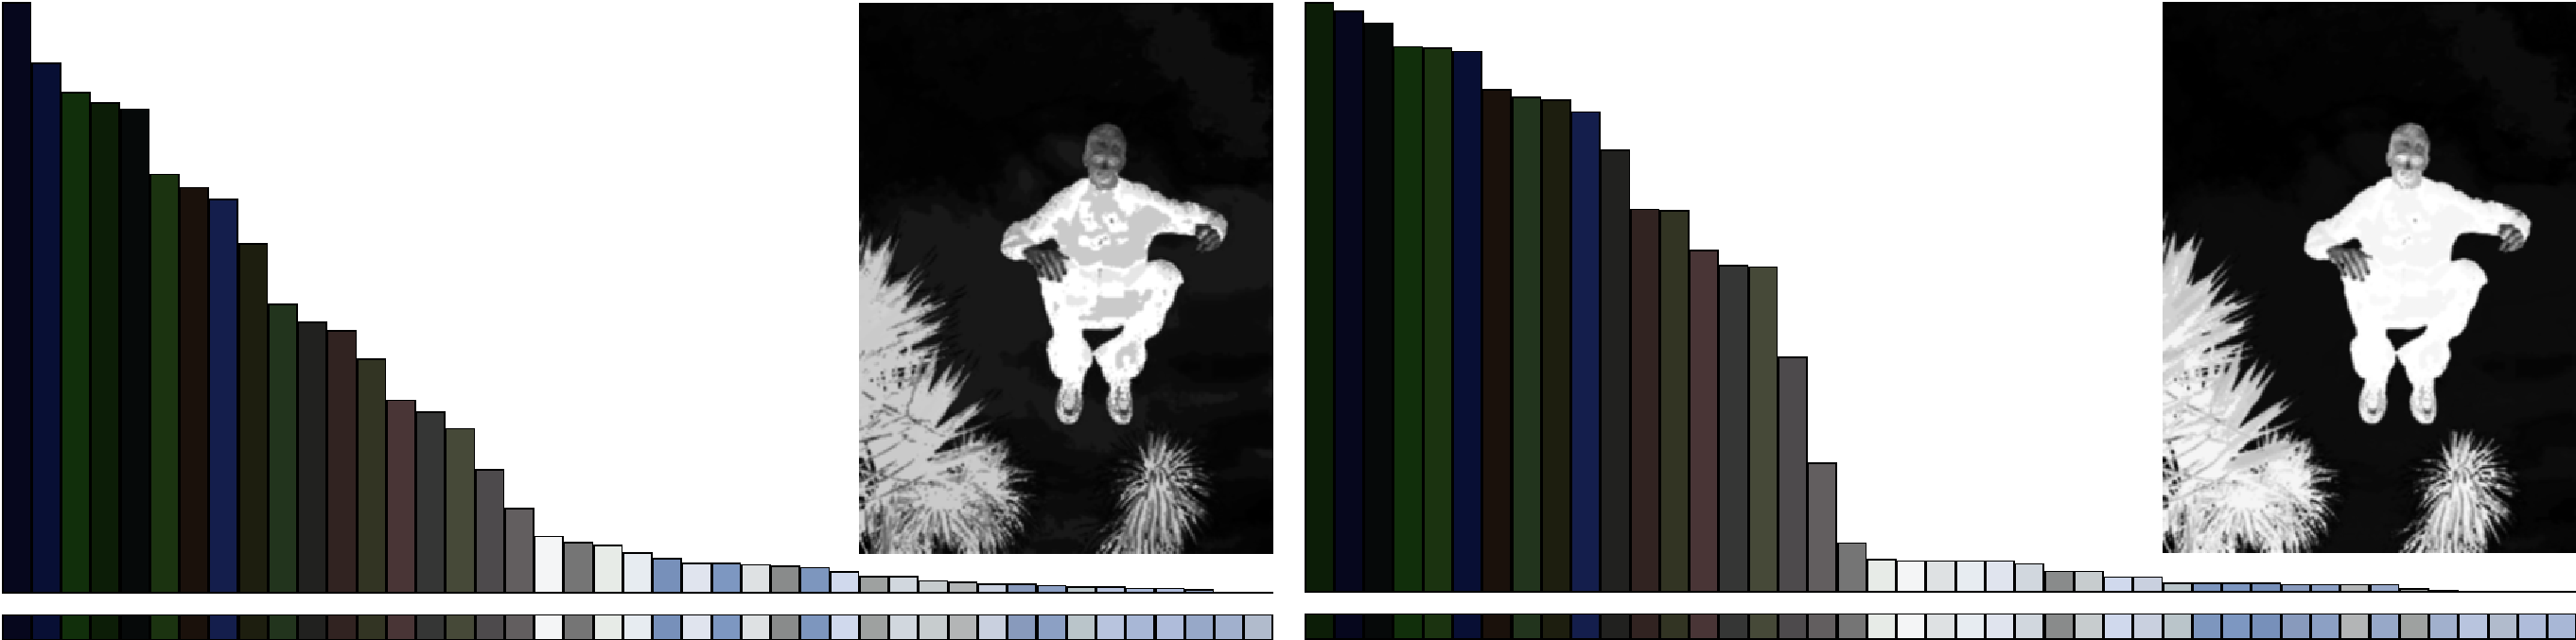
\includegraphics[width=\columnwidth]{histogram_saliency.pdf}
    \caption{颜色空间平滑前(左)后(右)像素颜色的显著性值
        (归一化到$[0, 1]$)。
        对应的显著性图在各自的内嵌插图中显示。
    }\label{fig:HCSmoothing}
\end{figure}

%%%%%%%%%%%%%%%%%%%%%%%%%%%%%%%%%%%%%%%%%%%%%%%%%%%%%%%%%%
\section{基于区域的对比度}

\begin{figure}[b]
    \centering
    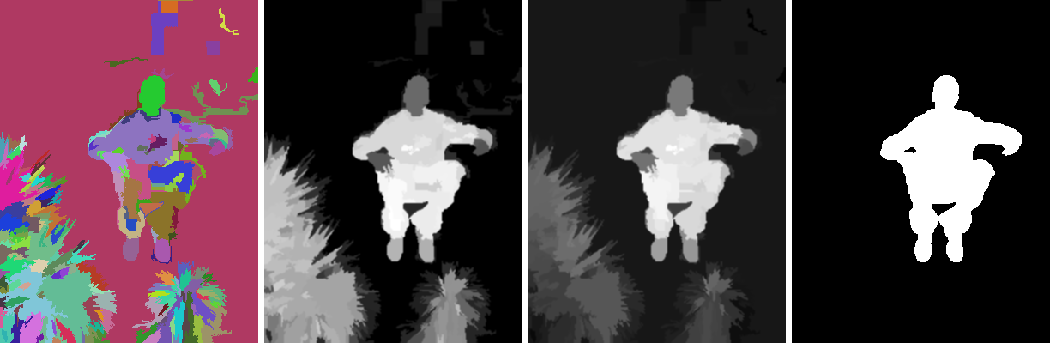
\includegraphics[width=\columnwidth]{region_contrast.pdf}\\
    \caption{由Felzenszwalb和Huttenlocher的分割方法
        \cite{04ijcv/felzenszwalb_efficient}得到的图像区域(左),
        考虑(中-右)和不考虑(中-左)距离权值分别得到的区域对比度。
        通过考虑空间关系,我们得到的高质量的重要性分割结果(右)可以和人工分割结果相比。
    }\label{fig:regContrast}
\end{figure}


\begin{figure*}[t]
   \begin{overpic}[width=\textwidth]{comparison.pdf} \small
   \put(3,0){(a)~original}
   \put(18.5,0){(b)~LC}
   \put(33,0){(c)~CA}
   \put(48,0){(d)~FT}
   \put(60,0){(e)~\HC}
   \put(74,0){(f)~\RC}
   \put(90,0){(g)~RCC}
   \end{overpic}
   \caption{显著性图的视觉效果对比。(a)原图,由以下方法产生的显著性图
       (b) Zhai和Shah\cite{06acmmm/ZhaiS_spatiotemporal},
       (c) Goferman等\cite{10cvpr/goferman_context},
       (d) Achanta等\cite{09cvpr/Achanta_FTSaliency},
       (e) 我们的HC和(f)RC方法,和(g)基于RC图的显著性区域分割结果.
       我们的方法的结果均匀的突出整个显著性区域。
       整个数据集上的所有检测结果可以从我们的项目主页上获取。
   }\label{fig:VisualComparison}
\end{figure*}


人们会更加注意到图像中和周围物体对比度非常大的区域
\cite{03neuroscience/luminanceContrast}。
除了对比度之外,空间关系在人类注意力方面也起到非常大的作用。
相邻区域的高对比度比很远区域的高对比度更容易导致一个区域引起视觉注意。
在计算像素级对比度时引进空间关系计算代价会非常大,
我们引进一种对比度分析方法:\emph{区域对比度} (Region Contrast, RC),
以此来将空间关系和区域级对比度计算结合到一起。
在RC方法中,我们首先将图像分割成若干区域,
然后计算区域及颜色对比度,再用每个区域和其它区域对比度加权和来为此区域定义显著性值。
权值由区域空间距离决定,较远的区域分配较小的权值。


%%%%%%%%%%%%%%%%%%%%%%%%%%%%%%%%%%%%%%%%%%%%%%%%%%%%%%%%%%
\mypara{用稀疏直方图比较来计算区域对比度}
首先,我们用基于图的图像分割方法将输入图像分割成若干区域
\cite{04ijcv/felzenszwalb_efficient}。
然后为每个区域建立颜色直方图\secref{sec:HC}。
对每个区域$r_k$,我们通过测量它与图像其它区域的颜色对比度来计算它的显著性值,
\begin{equation}\label{equ:regContrastSaliency}
    S(r_k) = \sum_{r_k \neq r_i} w(r_i)  D_r(r_k, r_i),
\end{equation}
其中$w(r_i)$为区域$r_i$的权值,$D_r(\cdot, \cdot)$为两个区域的颜色距离度量。
这里我们用 $r_i$里的像素数$w(r_i)$ 来强调大区域的颜色对比度。
两个区域$r_1$和$r_2$的颜色距离为:
\begin{equation}\label{equ:regContrast}
    D_r(r_1, r_2) = \sum_{i=1}^{n_1} \sum_{j=1}^{n_2} f(c_{1,i}) f(c_{2,j}) D(c_{1,i}, c_{2,j})
\end{equation}
其中$f(c_{k,i})$为第$i$个颜色$c_{k,i}$在第$k$个区域$r_k$的所有$n_k$种颜色中
出现的概率,$k=\{1,2\}$。
注意到我们使用区域的概率密度函数(即归一化的颜色直方图)中颜色出现概率作为权值,
以强调主要的颜色之间的区别。

因为每个区域只包含图像的直方图中很少数目的颜色,
所以为每个区域存储和计算常规矩阵形式的直方图是低效的。
我们用稀疏直方图以使得存储和计算过程更加高效。


%%%%%%%%%%%%%%%%%%%%%%%%%%%%%%%%%%%%%%%%%%%%%%%%%%%%%%%%%%

\begin{table*}
    \centering
    \begin{tabular}{l|c|c|c|c|c|c|c|c|c|c} \hline\hline
      方法  &  \IT   &  \MZ  &   \GB  &  \SR   &  \FT  &  \AC  &  \CA   & \LC   &  HC   &  RC   \\ \hline
      时间(秒) & 0.611  & 0.070 & 1.614  & 0.064  & 0.016 & 0.109 &  53.1  & 0.018 & 0.019 & 0.253 \\ \hline
      代码类型    & Matlab & C++   & Matlab & Matlab &  C++  &  C++  & Matlab &  C++  &  C++  &  C++  \\ \hline\hline
    \end{tabular}
    \caption{计算Achanta等人数据集\cite{09cvpr/Achanta_FTSaliency}中图像的平均用时。
        该数据集(参见我们主页)中大部分的图像分辨率为$400\times300$。
        这里所示的所有方法的时间是在一个拥有Dual Core 2.6 GHz
        CPU,2GB内存的机器上测得的。
    } \label{tab:TimeEfficency}
\end{table*}


\mypara{空间加权区域对比度 }
更进一步,通过在\equref{equ:regContrastSaliency}中引进空间权值,
我们将空间信息加入进来,来增加区域的空间影响效果。
近邻的区域增大影响,较远的区域减小影响。
特别地,对任意区域 $r_k$,基于空间加权区域对比度的显著性定义为:
\begin{equation}\label{equ:regContrastSpatial}
    S(r_k)=\sum_{r_k\neq r_i}\exp({-D_s(r_k,r_i)/\sigma_s^2})w(r_i) D_r(r_k, r_i)
\end{equation}
其中 $D_s(r_k, r_i)$ 为区域$r_k$ 和 $r_i$的空间距离,$\sigma_s$控制空间权值强度。
$\sigma_s$ 越大,空间权值的影响越小,导致较远区域的对比度会对当前区域显著性值做出较大的贡献。
两个区域的空间距离定义为两个区域重心的欧氏距离。在我们的试验中,$\sigma_s^2 = 0.4$,像素坐标归一化到$[0, 1]$区间。


%%%%%%%%%%%%%%%%%%%%%%%%%%%%%%%%%%%%%%%%%%%%%%%%%%%%%%%%%%%%%%%%%%%%%%
\section{实验比较}\label{sec:Experiment}


我们在Achanta等人提供的公开测试集\cite{09cvpr/Achanta_FTSaliency}上测试了我们的方法。
据我们所知,此测试集是此类数据最大的测试集,并且由人工精确标注了显著性区域。
我们将基于全局对比度的方法与其它$8$个当今最好的方法进行了比较。
仿照\cite{09cvpr/Achanta_FTSaliency},我们依据以下几个方面来选择其它方法来进行对比:
引用数(\IT ~和 \SR)、较新的方法(\GB, SR, \AC, \FT ~and \CA)、
多种类(IT 为生物驱动, \MZ~为纯计算, GB 为两者混合的, SR 在频域进行处理,
AC and FT 输出全分辨率显著性图),和我们方法最接近的(\LC)。


我们的方法和其它的方法在1000张图片上计算得到了显著性图。
\tabref{tab:TimeEfficency} 比较了每个方法的平均用时。
我们的方法HC和RC用C++实现,对于IT、GB、SR、FT和CA,我们引用了作者的实现。
由于找不到LC作者的源码,我们用C++来实现了此算法。
对于典型自然图片,HC 方法时间复杂度为 $O(N)$,对于实时应用已经非常高效。
相比之下,RC需要图像分割~\cite{04ijcv/felzenszwalb_efficient},
所以较慢,但它产生更好的效果。

\begin{figure*}[t]
  \centering
  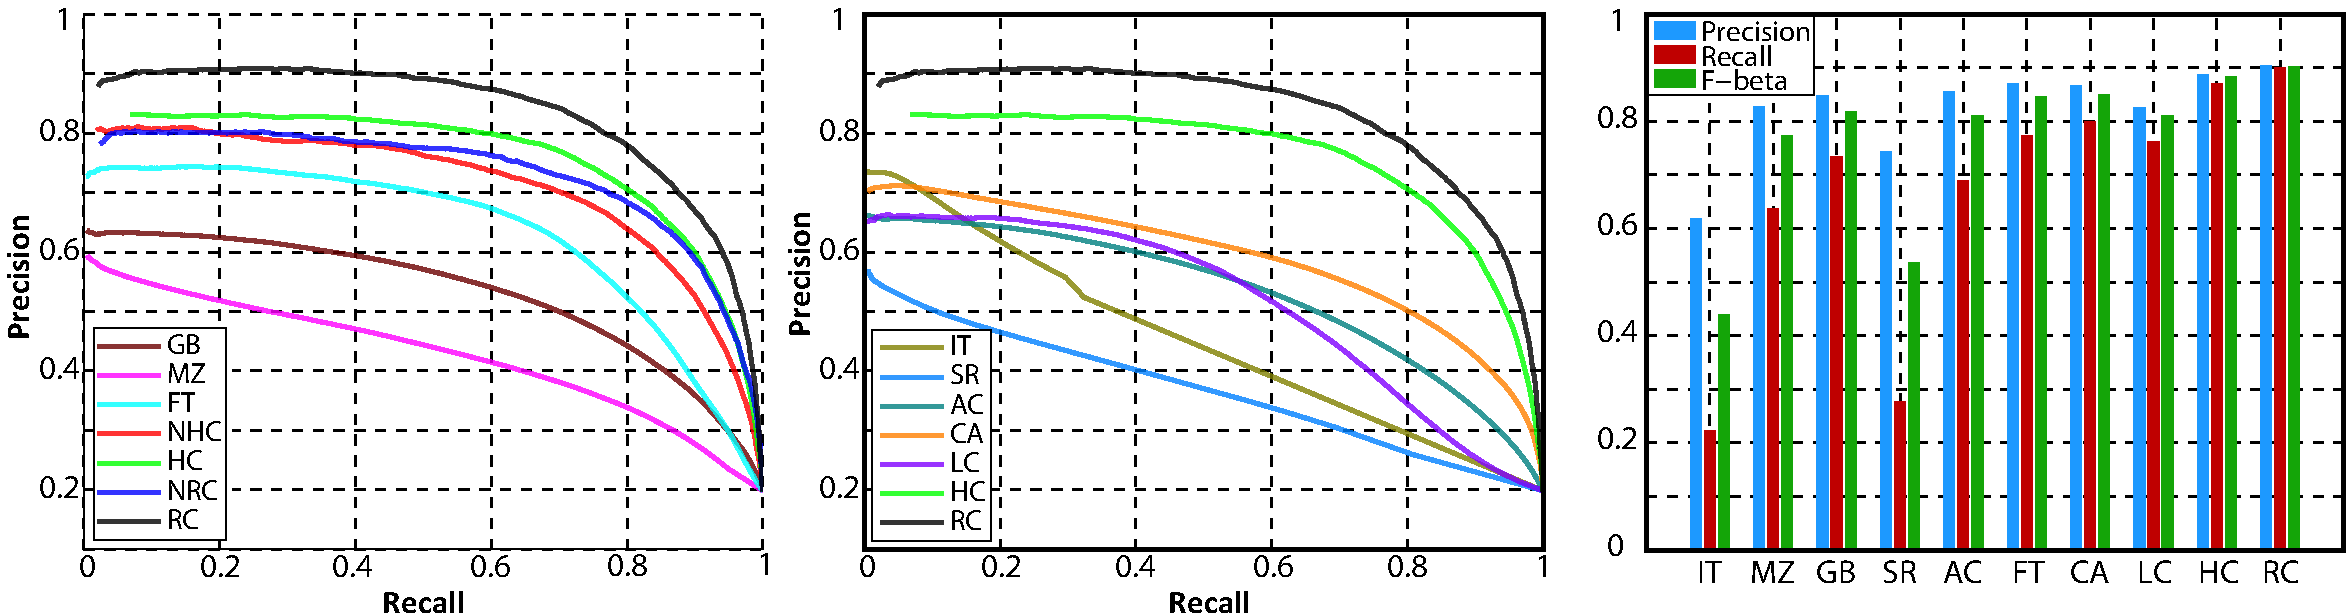
\includegraphics[width=\textwidth]{plots.pdf}
  \caption{在包含1000副图像的公开测试集上各种方法检测得到的显著性图经过
      简单阈值分割得到结果的正确率召回率曲线。
      左图和中图是我们方法不同配置与\GB, \MZ,  \FT, \IT, \SR, \AC, \CA,和\LC
      等方法的比较。
      NHC代表我们HC方法不带颜色空间平滑,NRC代表我们RC方法不带空间加权。
      右图是我们显著性区域分割方法以不同的显著性图作为初始值得到的正确率召回率柱状图。
      我们的RC方法在1000副图像数据集上的结果具高的精度,召回率和$F_{\beta}$值。
      (相关的结果图像从我们的项目主页上可以得到。)
  } \label{fig:plots}
\end{figure*}

为了全面的测试我们提出的方法的准确性,我们用了两种不同的客观比较方法进行了试验。
在第一个实验中,为了分割显著性物体并计算准确率召回率曲线,
我们参考\cite{09cvpr/Achanta_FTSaliency},用所有阈值分别将显著性图进行二值化。
在第二个试验中,我们用显著性图像初始化后迭代应用GrabCut方法
\cite{04tog/rother_grabcut}进行显著性物体分割。
我们还将得到的显著性图作为内容敏感的图像缩放和非真实感渲染的重要性权值。


%%%%%%%%%%%%%%%%%%%%%%%%%%%%%%%%%%%%%%%%%%%%%%%%%%%%%%%%%

\mypara{固定阈值的分割}
得到显著性物体的二值分割的最简单方法就是设定一个$T_f \in [0, 255]$的阈值。
为了可靠地比较多样的显著性检测方法高亮显著性物体的效果,
我们将阈值$T_f$设定为在$0$到$255$之间变化。\figref{fig:plots}为精确度召回率曲线结果。
我们还介绍了加入色彩空间平滑以及空间权值后的效果以及与其它方法的比较。
这些方法得到的显著性图的视觉直观比较在图~\ref{fig:cmp1vAll}
和图\ref{fig:VisualComparison}中。

正确率、召回率曲线清楚地展示出我们的方法优于其它的八种方法。
曲线的极限很有趣:在$T_f=0$处召回值最大,所有的像素被认为是前景,
所以所有的方法得到相同的正确值和召回值;这点的正确值为$0.2$,召回值为$1.0$。
这表明,在标注数据中,平均$20\%$的图像像素属于显著性区域。
曲线另一端,我们的方法的最小召回值比其它方法高,
因为我们的显著性图更加平滑,且包含更多显著性值为$255$的像素。


%%%%%%%%%%%%%%%%%%%%%%%%%%%%%%%%%%%%%%%%%%%%%
\mypara{显著性分割}
我们考虑将计算所得的显著性图像用于帮助显著物体分割。
在已有的工作中,显著性图已经被用于非监督物体分割:Ma和Zhang\cite{03ACMMM/Ma_Contrast-based}
通过在显著性图上进行模糊区域增长来找到矩形显著的区域。
Ko和Nam\cite{06josa/KoN_InterestSegmentation}在图像线段特征上训练支持向量机,
然后将这些区域聚类来提取显著性物体。
Han等人\cite{06TCSVT/han_unsupervised}用颜色、纹理和边缘特征建立马尔可夫
随机场模型,用显著性图的种子值来增长显著性物体区域。
最近,Achanta 等人~\cite{09cvpr/Achanta_FTSaliency}先通过mean-shift分割得到图像区域,
然后再图像区域内对显著性值进行平均,
再通过识别平均显著性值大于整个图像平均显著性值的2倍的图像区域来确定显著性区域。

\begin{figure}[b]
    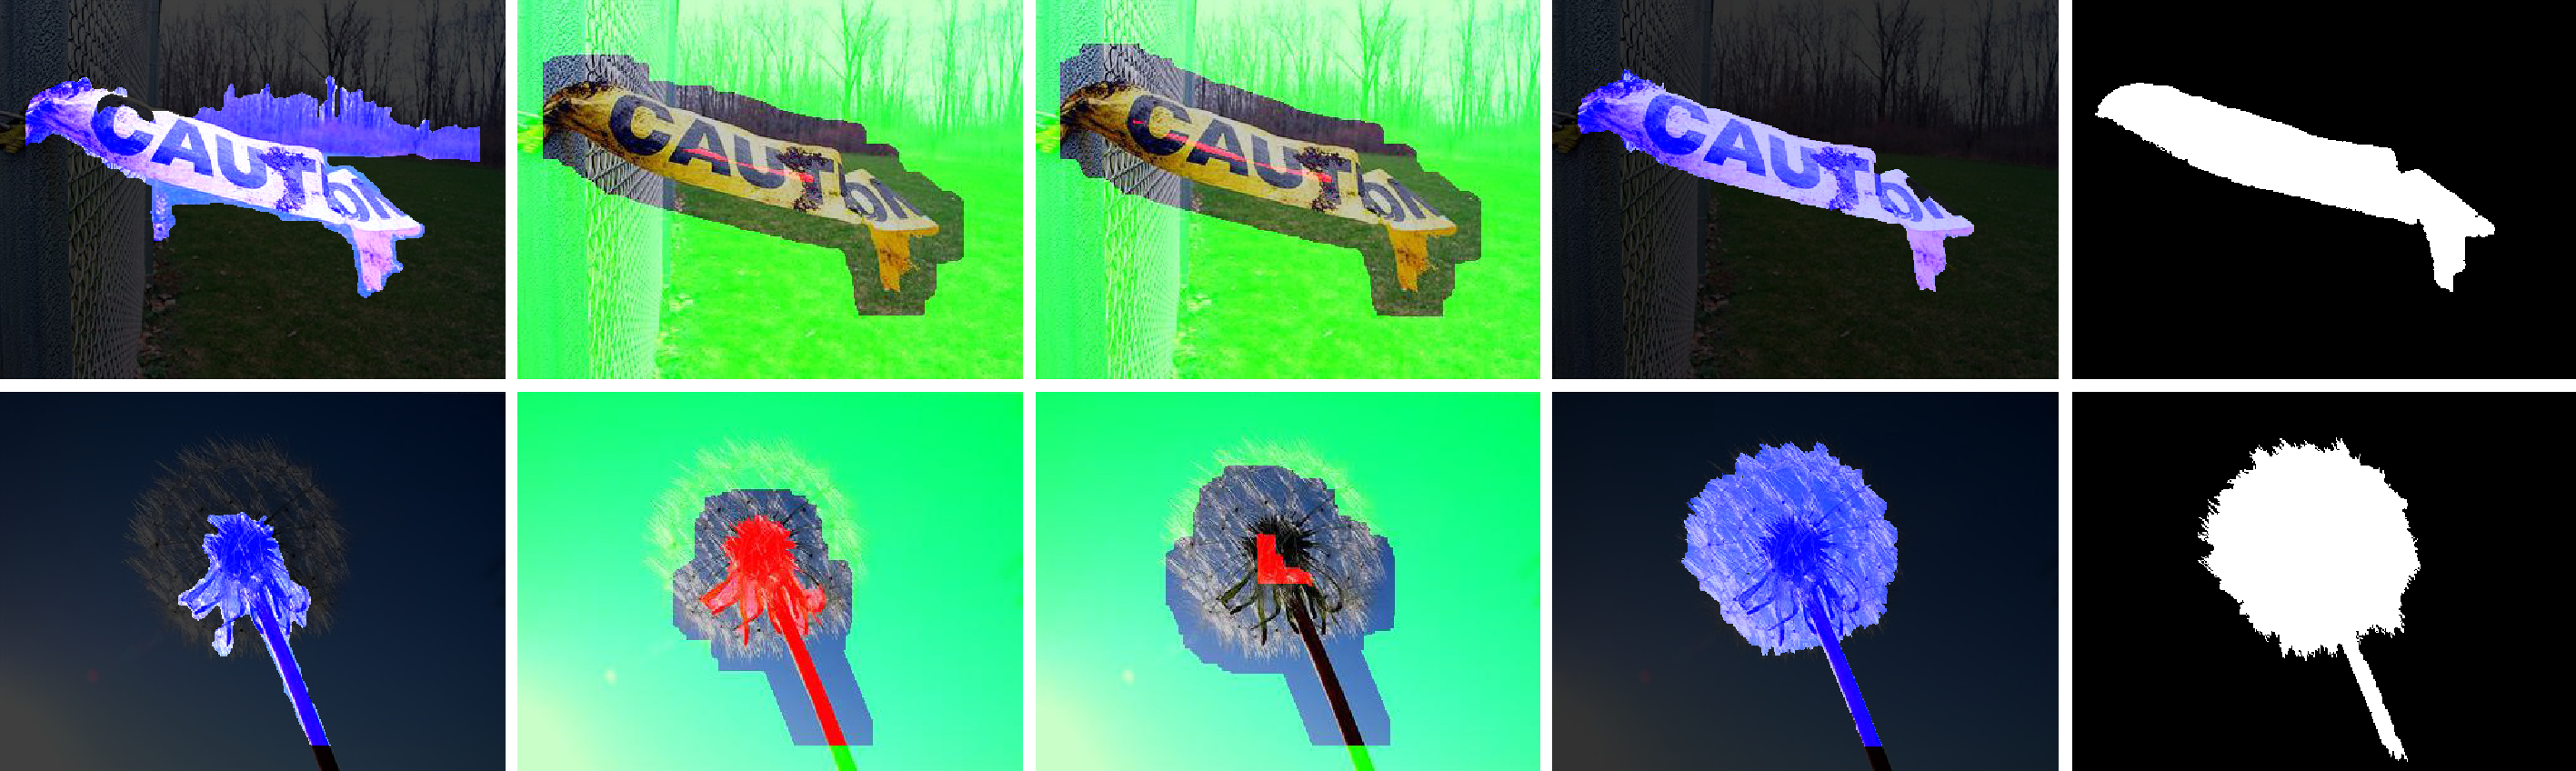
\includegraphics[width=\columnwidth]{saliency_cut.pdf}
    \caption{显著性区域分割。从左到右依次是:初始分割结果、第一次迭代后的trimap,
          第二次迭代后的trimap,最终分割结果,用户标注的基准数据。
          在分割图中,蓝色代表前景,灰色是背景。
          在trimap中,红色是前景,绿色是背景,未知区域为原图颜色。
    }\label{fig:AttCutSteps}
\end{figure}

\begin{figure*}
  \begin{overpic}[width=\linewidth]{cut_compare.pdf}\small
    \put(3,0){(a)~original}
    \put(17,0){(b)~\LC}
    \put(32,0){(c)~\CA}
    \put(46,0){(d)~\FT}
    \put(60,0){(e)~\HC}
    \put(74,0){(f)~\RC}
    \put(87,0){(g)~ground truth}
  \end{overpic}
  \caption{用不同显著性图初始化显著性分割的结果。相应的显著性图在
    \figref{fig:VisualComparison}中.
  }\label{fig:cutCmp}
\end{figure*}

在我们的方法中,我们迭代应用GrabCut \cite{04tog/rother_grabcut} 来改善二值化显著性
图像后得到的分割结果(见\figref{fig:AttCutSteps})。
传统的GrabCut方法是由人工选中矩形区域来进行初始化操作,
而我们用一个固定阈值二值化后的显著性图来得到显著性分割,
并用这个显著性分割来自动地进行GrabCut初始化。
这个阈值的我们经验性的选择固定阈值实验中与$95\%$召回率对应的阈值。


初始化之后,我们迭代运行GrabCut来改进显著性分割结果(在我们的实验中最多迭代 $4$ 次)。
在每一次迭代后,我们用膨胀和腐蚀操作来得到新的Trimap以进行下一次迭代。
如\figref{fig:AttCutSteps}所示,膨胀后仍然落在外面的区域设置成背景,
在腐蚀区域内的设置成前景,其余的区域为Trimap中的未知。
Grubcut本身是用高斯混合模型和Grapcut进行迭代,来改善每一步的区域分割效果,
靠近初始显著性物体区域的部分成为显著性物体的几率更大。
因此,我们的新的初始化方法可以使GrabCut包含显著性区域附近的显著性区域,
并根据颜色特征的差异排除非显著性区域。
在算法实现中,我们设置了狭窄的图像边界区域(15像素宽)作为背景来提高边界区域的收敛速度。


\figref{fig:AttCutSteps}展示了我们显著性分割算法的两个实例。
在旗子的例子中,不需要的区域被正确地排除;
在花朵的例子中,我们的方法扩展了初始显著性区域并收敛得到了精确的分割结果。
为了保持一致性,我们用召回率$95\%$的阈值对显著性图像进行二值化(见\figref{fig:plots})。
我们在基准数据集~\cite{09cvpr/Achanta_FTSaliency}上比较了平均正确率,召回率以及
$F$-测量,其中$F$-测量定义为:
\begin{equation}\label{equ:FMeasure}
    F_{\beta}= \frac{(1+\beta^2)Precision \times
        Recall}{\beta^2 \times Precision + Recall}.
\end{equation}

和Achanta等人\cite{09cvpr/Achanta_FTSaliency}一样,
我们用$\beta^2=0.3$来使正确率的权重高于召回率。
可以从比较结果(见\figref{fig:plots}-右和\figref{fig:cutCmp})中看出,
用我们的 RC 和 HC 显著性图来进行分割明显优于其它方法。
和当今最好的方法相比(正确率=$75\%$, 召回率=$83\%$),我们方法的结果更精确
(正确率=$90\%$, 召回率=$90\%$)。
(我们的演示程序可以从项目主页中得到。)


%%%%%%%%%%%%%%%%%%%%%%%%%%%%%%%%%%%%%%%%%%%%%%%%%%%%
\begin{figure}[t!]
   \begin{overpic}[width=\columnwidth]{contentAware_application.pdf} \small
   \put(3,0){original}
   \put(21,0){CA}
   \put(31,0){RC}
   \put(48,0){original}
   \put(75,0){CA}
   \put(90,0){RC}
    \end{overpic}
    \caption{用\CA 和我们的RC显著性图进行内容敏感的图像缩放
        \cite{09cgf/ZhangC}的结果比较。
    }\label{fig:Resizing}
\end{figure}


\mypara{基于内容感知的图像缩放}
在内容敏感的图像缩放中,显著性图像经常用来指定图像的相对重要区域
(见~\cite{09_image_resize})。
我们用提取出的显著性图像进行了图像缩放实验。
实验中采用了Zhang等人提出的\cite{09cgf/ZhangC}内容敏感图像缩放方法
\footnote{我们采用作者公开的代码}。
该方法通过变形能量将变形分配到相对非显著性区域,同时保持全局和局部的图像特征。
\figref{fig:Resizing}比较了用\RC 和\CA 显著性图像得到的图像缩放结果。
显著性物体区域的显著性值是成片光滑的,这点对于基于能量的缩放非常重要,
因此我们的 RC 显著性图产生更好的缩放结果。
CA显著性图像在物体的边界有更高的显著性值,但这并不适于图像缩放等应用,
这些应用要求整个显著性物体一致的被突出。


%%%%%%%%%%%%%%%%%%%%%%%%%%%%%%%%%%%%%%%%%%%%%%%%%
\mypara{非真实感渲染}
艺术家们经常对图像抽象并突出有意义的部分并掩盖非重要区域\cite{99/zeki_innerVision}。
受此现象启发,一系列用显著性值来进行非真实感渲染的方法产生,
并产生了有趣的结果~\cite{02tog/decarlo_stylization}。
我们将我们的方法和最近的杰出的显著性检测方法~\cite{09cvpr/Achanta_FTSaliency}用在NPR
技术\cite{10pg/Huang_Zhang}上进行了比较(见\figref{fig:NPR})。
我们的\RC 提供更好的掩模,这可以帮助NPR方法更好地保留重要图像部分以及区域边界的细节,
同时平滑其它部分。


%%%%%%%%%%%%%%%%%%%%%%%%%%%%%%%%%%%%%%%%%%%%%%%%%%%%
\begin{figure}[t!]
   \begin{overpic}[width=\columnwidth]{npr_application2.pdf} \small
     \end{overpic}
    \caption{(左,右)~\FT 和RC显著性图分别被用于风格化绘制\cite{10pg/Huang_Zhang}。
        我们的方法生成了更好的显著性图,是的风格化绘制保持了重要部分的细节。例如马头
        和栏杆部分细节更好的保留了。
    }\label{fig:NPR}
\end{figure}


\begin{figure}[t!]
   \begin{overpic}[width=\columnwidth]{challenging_maps.pdf} \small
     \end{overpic}
    \caption{对于我们提出的基于直方图的方法来说一个有挑战性的例子:(上图)显著性区域和
        非显著性区域具有相似的颜色,(下图)图像具有复杂的纹理背景。
        从左到右依次是输入图像、HC显著性图、HC显著性区域分割、RC显著性图、 RC显著性区域分割.
    } \label{fig:challenging_maps}
\end{figure}



%%%%%%%%%%%%%%%%%%%%%%%%%%%%%%%%%%%%%%%%%%%%%%%%%

\section{总结与展望}\label{sec:Conclusion}
我们提出了基于全局对比度的显著性计算方法,即基于直方图对比度~(HC) 和基于空间信息增强的区域对比度~(RC)方法。
HC方法速度快,并且产生细节精确的结果,RC方法可以产生空间增强的高质量显著性图像,但与此同时具有相对较低的计算效率。
我们在国际上现有最大的公开数据集上测试了我们的方法,并与之前已有八种最好的其它方法进行了比较。
实验结果表明,我们提出的方法在正确率和召回率上都明显优于其它方法,并且简单而高效。

在未来的工作中,我们计划研究包含空间关系且保留详细细节的显著性图像的高效计算算法,
并且希望研究能够处理具有复杂纹理的背景图像的显著性检测算法,
以克服我们现有算法在处理这类情况中存在的缺陷。
最后,我们还希望显著性图像的检测过程中进一步考虑人脸、对称性等高级因素。
我们相信显著性图像可以应用于高效物体检测\cite{06TCSVT/han_unsupervised},
可靠图像分类,鲁棒的图像景物分析~\cite{journal/tog/ChengZMHH10},
并提高图像检索效果\cite{tog09/ChenCT_Sketch2Photo}。


\paragraph{致谢.} 本项目受到了国家973计划(2011CB302205), 国家863计划(2009AA01Z327),
国家自然科学基金(U0735001),以及国家核高基计划(2011ZX01042-001-002)的支持.
程明明的工作受到了Google PhD fellowship, IBM PhD fellowship, 以及教育部博士研究生学术新人奖的资助。

{\small
\bibliographystyle{ieee}
\bibliography{Saliency}
}

% \end{CJK*}
\end{document}
